\documentclass[11pt, a4paper]{beamer}
\usepackage{amsmath}
\usepackage{amsfonts}
\usepackage{amssymb}
\usepackage{tikz}
\usetheme{Frankfurt}
\usecolortheme{seagull}
\usepackage{xltxtra,fontspec}
\usepackage{polyglossia}
\setmainlanguage{english}
\defaultfontfeatures{Scale=MatchLowercase}

\usepackage[absolute,overlay]{textpos}

\setbeamertemplate{footline}
{
  \leavevmode%
  \hbox{%
  \begin{beamercolorbox}[wd=.6\paperwidth,ht=2.25ex,dp=1ex,center]{author in head/foot}%
    \usebeamerfont{author in head/foot}\insertshortauthor
  \end{beamercolorbox}%
  \begin{beamercolorbox}[wd=.4\paperwidth,ht=2.25ex,dp=1ex,center]{title in head/foot}%
    \usebeamerfont{title in head/foot}\insertshorttitle\hspace*{3em}
    \insertframenumber{} / \inserttotalframenumber\hspace*{1ex}
  \end{beamercolorbox}}%
  \vskip0pt%
}


\setbeamertemplate{navigation symbols}{}

\author{Dan Häberlein, Peggy Lucke, J. Nathanael Philipp, Alexander Richter}
\title[The openLegislature project]{Current Topics in Digital Philology\\The openLegislature project}
\date{}
\institute{Universität Leipzig}

%\logo{\includegraphics[scale=0.25]{./LGD_Logo.png}}
%\setbeamersize{text margin left=7mm, text margin right=7mm}

%\usepackage[babel]{csquotes}
%\defbibheading{bibliography}{}
%\bibliography{quellen}

\usepackage[backend=biber,style=numeric]{biblatex}
\addbibresource{lit.bib}

\begin{document}
\section{}
\begin{frame}
\titlepage
\end{frame}

\only<presentation| handout:0> {
	\AtBeginSection[]{%
		\begin{frame}
		\frametitle{Outline}
		\tableofcontents[currentsection]
		\end{frame}
	}% AtBeginSection
}

\only<2| handout:1>{
	\begin{frame}
		\frametitle{Outline}
		\tableofcontents
	\end{frame}
}

\section{Introduction}
\subsection{Corpus}
\begin{frame}{Informations}
\textbf{Plenary Protocols from Bundestag}
\begin{itemize}
\item stenographic reports in PDF
\item open to the public
\item siehe bundestag.de \cite{bundestag} \\[1em]
\item size of corpus circa 10GB $\rightarrow$more than 3900 PDF 
\end{itemize}
\end{frame}

\subsection{Questions}
\begin{frame}{Questions to the information in the corpus}
\textbf{Statistic:}
\begin{itemize}
\item How many speakers are in one legislative period/total?
\item How many speeches from one party/speaker?
\end{itemize}
\textbf{Keyword-search:}
\begin{itemize}
\item Which speaker spoke to a special topic?
\end{itemize}
\textbf{Why this questions?}\\
We want more transparency! The answers are there, but too difficult to reach for all other people. That will be changed!
\end{frame}

\section{Methods} 
\begin{frame}{Methods}
\textbf{Preprocessing:}
\begin{itemize}
\item stop word filter
\item lower case transformation
\item word count for SLDA
\item tf-idf for log-likelihood
\item cooccurrences per speaker
\end{itemize}
\end{frame}

\begin{frame}
\frametitle{Methods}
\textbf{Algorithms:}
\begin{itemize}
\item Log-likelihood
\item Topic Modell / SLDA
\end{itemize}
\textit {"Latent Dirichlet allocation (LDA) is a generative probabilistic
	model of a corpus. The basic idea is that documents are represented as
 	random mixtures over latent topics, where each topic is characterized by a
 	distribution over words."}, siehe \cite{blatent}
%  	

\textit{In supervised latent Dirichlet allocation (sLDA), we add to LDA a response variable associated with each document}, \cite{BleiSupervisedTopicModels}
\end{frame}

\begin{frame}{SLDA Methods}
\begin{enumerate}
\item single step approach
\begin{itemize}
\item create single dataset for an election period
\item calculate top words for each speaker
\end{itemize}
\item two step approach
\begin{itemize}
\item create dataset for each protocol
\item calculate top words for each speaker
\item merge results for an election period
\item calculate top words for each speaker
\end{itemize}
\end{enumerate}
\end{frame}

\begin{frame}
  \frametitle{Architectural process for data extraction and preparation}
  \begin{itemize}
  \item Usage of Listener Patterns \cite{javainsel9}
  \item Usage of Github-Library Async \cite{async} for easy creation of concurrent process chains
  \end{itemize}  
  \begin{center}
    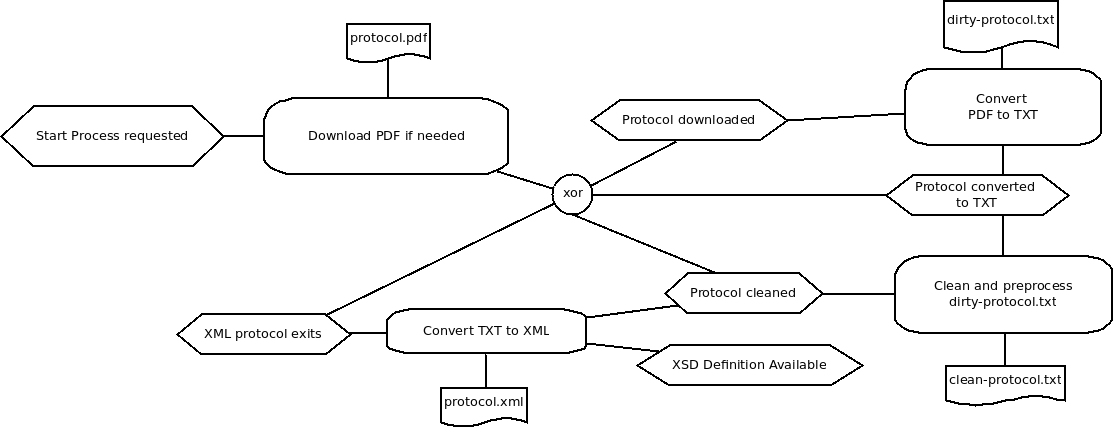
\includegraphics[width=1\textwidth]{../../doc/process-overview.png}
  \end{center}
\end{frame}


\section{Results}
\begin{frame}
\frametitle{temporary results}
\begin{itemize}
\item unstructured Textfiles avaiable (PDF / TXT) for all election periods
\item semi-structured XML files processed from PDF
\item Metadatabase (NEO4J) with data of all election periods
\item XPath query's on XML-Files
\end{itemize}
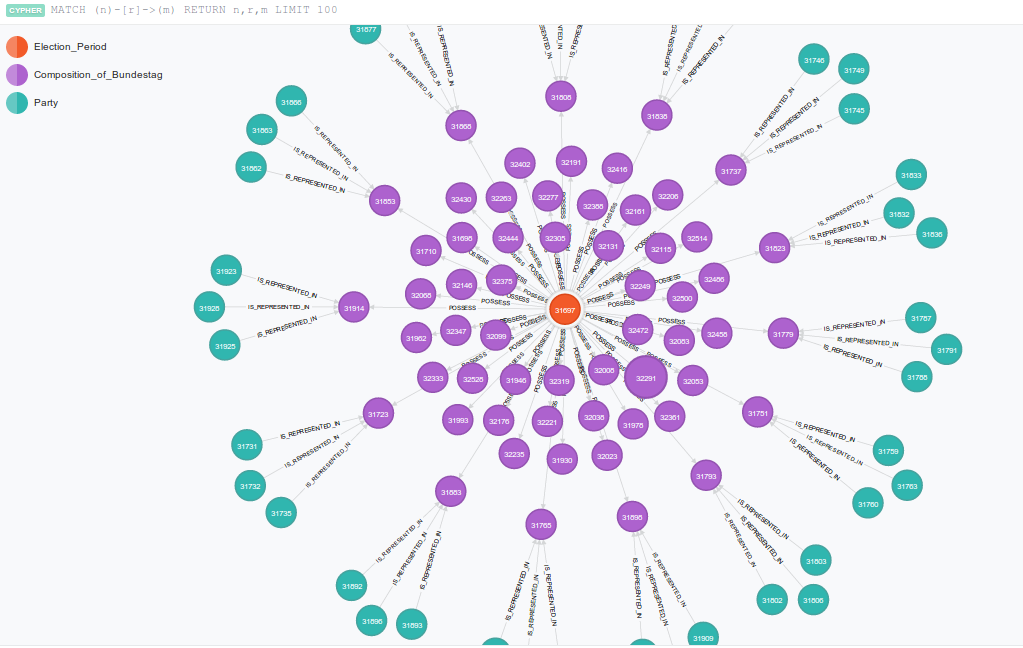
\includegraphics[scale=0.25]{metadatabase.png}
\end{frame}

\begin{frame}
\frametitle{temporary results 2}
\begin{itemize}
\item NoSQL Database:
	\begin{itemize}
		\item all speeches
		\item Speaker with all Speeches
		\item appearance of words by speech
		\item Speakerstatistics over all election periods
		\item Partystatistics over all election periods
	\end{itemize}
\item website for browsing corpusdata/-statistics with visualisations
\item imput files for slda (arff-files) generated ( for 18th election period )
\item slda output: significant words for each speaker of the 18th election period 
\end{itemize}
\end{frame}

\begin{frame}
\frametitle{Statistics}
\begin{itemize}
\item 18 election periods
\item 7004 speaker
\item 679910 speeches
\item 39 partys
\item But: data not as clean as possible
\begin{itemize}
\item typing errors: e.g. "CSU/CSU", "Pawelcyzk" "Pawelczyk" "Pawelzcyk"
\item parsing problems
\end{itemize}
\end{itemize}
\end{frame}

\begin{frame}
\frametitle{Statistics 2: Speeches pro election period}
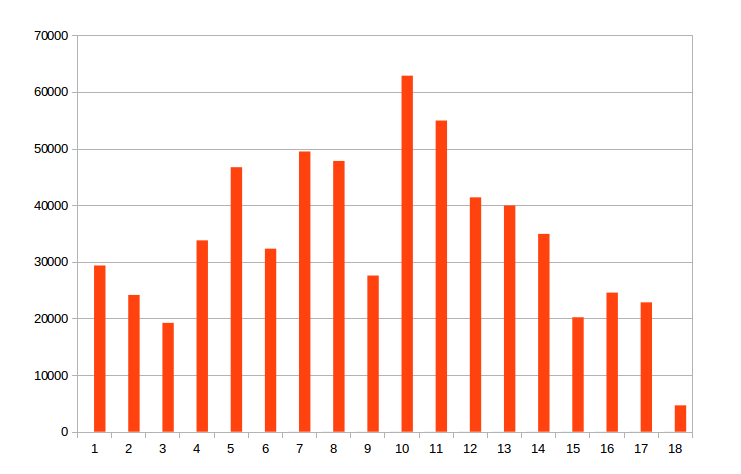
\includegraphics[scale=0.4]{speechperperiod.png}
\end{frame}

\begin{frame}
\frametitle{significant words for speeches}
18th election period, second session: Thomas Oppermann
\begin{itemize}
\item 1. staat
\item 2. verhandeln
\item 3. snowden
\item 4. nsa
\item 5. praxis
\item 6. geheimdienste
\item 7. ausspioniert
\item 8. hören
\item 9. möglichkeit
\item 10. schutz
\end{itemize}
\end{frame}

\begin{frame}
\frametitle{significant words for speeches 2}
18th election period, third session: Oskar Lafontaine
\begin{itemize}
\item 1. waffenexporte
\item 2. währung
\item 3. ökonomisch
\item 4. zukunftsaufgaben
\item 5. währungsspekulation
\item 6. übernachtungen
\item 7. verteilung
\item 8. waggons
\item 9. zug
\item 10. schneller
\end{itemize}
\end{frame}

\section{Outlook}

\subsection{next Steps}
\begin{frame}
\frametitle{What are our next tasks we need to accomplish?}
\begin{itemize}
	\item finalize our results, make them human accessable
	\item provide (easy) query interface for everyday users
	\item extend statistical webpage
\end{itemize}
\end{frame}

\begin{frame}
\frametitle{Last steps until the end of the semester}
\begin{itemize}
	\item reprocess xml parsing
	\item finish result visualization 
	\item connect our data with the meta data database (e.g. match every speeker to gouvernment / opposition)
	\item Log Likelihood on the GPU with our corpus
\end{itemize}
\end{frame}

\section{Take a chance on us!}
\begin{frame}
\frametitle{Take a chance on us!}
Our project could be really interessting in the following sence:
\begin{itemize}
\item History / Political Science  
\item Educational Purposes
\item Parties 
\end{itemize}
We would try to contact the listed stakeholder to learn more about there needs.\\

Also, we would like to distribute our resuls in a way that everybody can consume them. 
This could involve the enhancement of your current result page (namely by a query interface for keywords) or the 
administration of a virtual machine with our results and software artifacts to recreate them.
\end{frame}

\begin{frame}
\frametitle{What does it tell about humen history and society?}
\begin{itemize}
\item We could create deeper insights of how humens interact with each other, especially when they argue.
\item We can follow and study important milestones of history (from the European Coal and Steel Community to the European Union)
\item We can analyse which party and even which politian represents a specific opinion.
\end{itemize}
We think in the time of NSA and total surveillance a project like ours could contribute as a weapon against inresponsible politicians. 
The information about what the elected leaders actually do and say could be one step to a more enlightened society.

\end{frame}

\printbibliography

\end{document}
